\documentclass[frontgrid,a4paper]{flacards}
\usepackage{color}
\usepackage{mathtools}
\usepackage{amsmath}
\usepackage{amssymb}

\definecolor{light-gray}{gray}{0.75}
\fboxsep=20pt

\newcommand{\frontcard}[1]{\fboxsep=2pt\textcolor{light-gray}{\colorbox{light-gray}{$#1$}}}
\newcommand{\backcard}[1]{#1}
\newcommand\tab[1][0.5cm]{\hspace*{#1}}

\newcommand{\flashcard}[1]{% create new command for cards with blanks
    \card{% call the original \card command with twice the same argument (#1)
        \let\blank\frontcard% but let \blank behave like \frontcard the first time
        #1
    }{%
        \let\blank\backcard% and like \backcard the second time
        #1
    }%
}

\begin{document}

\pagesetup{2}{4}

\card{
  What does $O(<expr>)$ mean?
}{
  The complexity (i.e. running time/space) is bounded by the $<expr>$.
}

\card{
  What does $\Theta(<expr>)$ mean?
}{
  The complexity (i.e. space/running time) has the complexity proportional to
  $<expr>$.
}

\card{
  What does $\Omega(<expr>)$ mean?
}{
  The complexity (i.e. running time/space) is \textit{at least} by the $<expr>$.
}

\card{
  What are the best, average and worst case complexities of \textbf{Bubble Sort}?
}{
  Best: $O(n)$,\\ Average: $O(n^2)$,\\ Worst: $O(n^2)$
}

\card{
  What are the best, average and worst case complexities of \textbf{Merge Sort}?
}{
  Best: $O(n\log_2n)$,\\ Average: $O(n\log_2n)$,\\ Worst: $O(n\log_2n)$
}

\card{
  Give pseudo code for merging 2 sorted lists, as part of merge sort.
}{
  \begin{flushleft}
    Merge($L_1$, $L_2$) \\
    \tab if $L_1 = []$ return $L_2$ \\
    \tab if $L_2 = []$ return $L_1$ \\
    \tab $x_1 = L_1 [0]$ \\
    \tab $x_2 = L_2 [0]$ \\
    \tab $L'_1 = L_1 [1 : \vert L_1 \vert - 1]$ \\
    \tab $L'_2 = L_2 [1 : \vert L_2 \vert - 1]$ \\
    \tab if $x_1 \leq x_2$ \\
    \tab \tab return $[x_1]+$Merge($L'_1$ ,$L_2$) \\
    \tab return $[x_2]+$Merge($L_1$ ,$L'_2$)
  \end{flushleft}
  \textit{Merge two sorted lists}
}

\card{
  Give pseudo code for MergeSort(L).
}{
  \begin{flushleft}
    MergeSort(L) \\
    \tab if $\vert L \vert \leq 1$ \\
    \tab \tab return L \\
    \tab Split L into roughly equal halves, $L_l$ and $L_r$ \\
    \tab return Merge(MergeSort($L_l$),MergeSort($L_r$))
  \end{flushleft}
  \textit{MergeSort(L)}
}

\card{
  What are the best, average and worst case complexities of \textbf{Quick Sort}?
}{
  Best: $O(n\log_2n)$,\\ Average: $O(n\log_2n)$,\\ Worst: $O(n^2)$
}

\card{
  What would the pseudo code be for Quick Sort?
}{
  \begin{flushleft}
    quicksort(L) \\
    \tab if length of $L \leq 1$ \\
    \tab\tab return L \\
    \tab remove the first element, x, from L \\
    \tab $L_\leq :=$ elements of L less than or equal to x \\
    \tab $L_> :=$ elements of L greater than x \\
    \tab $L_l :=$ quicksort($L_\leq$) \\
    \tab $L_r :=$ quicksort($L_>$) \\
    \tab return $L_l$ + [x] + $L_r$ \\
  \end{flushleft}
  \textit{Quick Sort}
}

\card{
  Say that the input represents a positive integer, $x$, what is the size of $n$?
 }{
  $\left \lfloor \log_b x \right \rfloor + 1$
  Where $b$ is the number representation, usually binary (so 2).
 }

\card{
  What does it mean by $O(1)$?
}{
  It takes a constant time, no matter the amount of data, to perform the operation.
}

\card{
  What is the minimum time for any sorting algorithm that uses only number comparisons?
}{
  $n\log_2n$
}

\card{
  What would the pseudo code be for Euclid's algorithm?
}{
  \begin{flushleft}
    // Assume $a>=b$ \\
    hcf(a,b) \\
    \tab if $b = 0$ \\
    \tab\tab return a \\
    \tab $r=amodb$ \\
    \tab return hcf(b,r)
  \end{flushleft}
  \textit{Euclid's algorithm}
}

\card{
  What would the pseudo code be for Fast Modular Exponentiation?
}{
  \begin{flushleft}
    fme(a,b,k) \\
    \tab $d=a$ \\
    \tab $e=b$ \\
    \tab $s=1$ \\
    \tab While $e>0$ \\
    \tab\tab if e is odd \\
    \tab\tab\tab $s=(s.d)mod k$ \\
    \tab\tab $d = d^2 mod k$ \\
    \tab\tab $e = \lfloor e / 2 \rfloor$ \\
    \tab return s \\
  \end{flushleft}
  \textit{Fast Modular Exponentiation}
}

\card{
  What are some of the advantages of ElGamal encryption?
}{
     Sender Verification \\
     Private key remains with owner \\
     Public key is freely distributable \\
     No secret channel needed at any point \\
     No need for pre-shared keys
}

\card{
  What is the basic procedure for an encryption and decryption using publik key
  cryptography if Alice wants to send a message to Bob?
}{
  Alice generates a private random integer a and Bob generates a private
  random integer b \\
  Alice generates her public value $g^a \bmod{p}$ \\
  Bob generates his public value $g^b \bmod{p}$ \\
  Alice computes $g^{ab} = (g^a)^b \bmod{p}$ \\
  Bob computes $g^{ba} = (g^b)^a \bmod{p}$ \\
  Now they have a shared secret $k$ since $k = g^{ab} = g^{ba}$
}

\card{
  Describe public key generation in ElGamal encryption using p as the Prime
  Modulus and g as the Primitive root (as described in the COMP26120 lab)
}{
  Generate a large $p$ and a $g$ in $1 \leq g < p$ \\
  Generate a random integer $a$ in $1 \leq a \leq p - 2$ \\
  Compute $g^a \bmod{p}$. The public key is
  $$(p, g, g^a)$$
  The private key is $a$
}

\card{
  Describe the encryption procedure used in the ElGamal cryptosystem given that
  person B wants to send message M to preson A
}{
  Obtain A's public key $(p, g, g^a)$ \\
  Represent the message M as integers in the range ${0, ..., p - 1}$ \\
  Select a random integer k from $1 \leq k \leq p - 2$ \\
  Compute $\gamma = g^k \bmod{p}$ and $\delta = m \cdot (g^a)^k$ \\
  Send ciphertext $c = (\gamma, \delta)$ to A
}

\card{
  Describe the decryption process used in the ElGamal cryptosystem given that
  person A has received cyphertext $(\gamma, \delta)$ from person B, encrypted
  encrypted using the public key $(p, g, g^a)$
}{
  Use private key a to compute $(\gamma^{p-1-a}) \bmod{p}$ \\
  NOTE THAT: $(\gamma^{p-1-a}) = \gamma^{-a} = g^{-ak}$ \\
  Recover the message M by computing $(\gamma^{-a} \cdot \delta \bmod{p})$ \\
  Note that this evaluates to $(g^{-ak} \cdot g^{ak} \cdot M \bmod{p})$ or
  $1 \cdot M \bmod{p}$
}

\card{
  Consider the equation $a^x = y \bmod{p}$. If $a$ is a primitive root of modulo $p$, then for every $y (1\leq y < p)$, such an $x (1\leq x < p)$ exists. What is $x$?
}{
  X is the \textbf{discrete logarithm} of $y$ with base $a$, modulo $p$.
}

\flashcard{The \blank{discrete logarithm} is the inverse of exponentiation.}

\card{
  Why can a private key in the ElGamal cryptosystem not, in practice, be recovered
  using the public key when $p$ is large?
}{
  To calculate a public key, $y$, a private key, $x$ is needed. The equation for
  modular exponentiation can be used to generate the public key: $y = g^x \bmod{p}$
  where $g$ is a primitive root of the modulus $p$. \\
  It is considered a one-way, or trapdoor function - easy to compute, hard to invert.
  For a large $p$, one of the few ways to figure out the private key x would be to calculate
  $g^x \bmod{p}$ for every $x$ in $1 \leq x < p$ and find when one of these results matches $y$
}

\card{
  What is one way you can argue correctness of Euclid's algorithm?
}{
  Let $r = a mod b$. $hcf(a,b)=hcf(b,r)$ because all factors of a and b are also factors of b and r and vice versa. If they have the same factors, they have the same highest common factor.
}

\card{
  What would half the correctness proof be for Euclid's algorithm?
}{
  As $r=a \bmod{b}$, $\exists q$ such that $a=bq+r$, $\therefore r = a-bq$. \\
  Suppose x is a factor of a and b, then $\exists y and z$ such that $a=xy$, $b=xz$. \\
  Hence: $r=xy-xzq$, $r=x(y-zq)$. \\
  $\therefore x$ is a factor of r (and also of b and r).
}

\flashcard{
  $(a.b)modk=$ \blank{$(amodk.bmodk)modk$}
}

\card{
  Let $p$ be a prime number. What is meant by a primitive root modulo $p$?
}{
  The numbers $r_x$ between 1 and $p-1$ that, when raised by the numbers between 1 and $p-1$ compute all the numbers between 1 and $p-1$ in some order with no repetitions.
}

\card{
  What does saying that algorithm A runs in time g mean?
}{
  Given an input of size n, the number of operations executed by A is bounded above by g(n).
}

\card{
  What is a permutation of a set?
}{
  A 1-to-1 map of the set onto itself. In basic terms, it is a set mapped to
  another order of itself. i.e $[0,1,2,3,4] \mapsto [2,4,1,0,3]$
}

\card{
  What do we mean by a composition of two permutations?
}{
  The composition is the product of two permutations, $\alpha$ and $\beta$, on a set
  n, given by $\alpha \cdot \beta (n)$ or $\beta (\alpha(n))$
}

\card{
  What is the number of possible permutations on an n-element set?
}{
  $n!$
}

\card{
  In the context of a permutation, what do we mean by a transposition?
}{
  A transposition is a special kind of permutation where only 2 elements in
  a set are affected (they are swapped). On a set $X$ a transposition
  $\sigma = (i, j)$ is given by
  \[ \sigma(k) =
    \begin{cases}
      j  & \quad \text{if k = i}\\
      i  & \quad \text{if k = j}\\
      k  & \quad \text{ow.}
    \end{cases}
  \]
}

\card{
  Convert this pair of simultaneous equations into matrix form \\
  $a_{1,1} x_1 + a_{1,2} x_2 = b_1$\\
  $a_{2,1} x_2 + a_{2,2} x_2 = b_2$
}{
\[
 \begin{pmatrix}
  a_{1,1} & a_{1,2} \\
  a_{2,1} & a_{2,2}
 \end{pmatrix}
 \begin{pmatrix}
  x_{1} \\
  x_{2}
\end{pmatrix} =
\begin{pmatrix}
  b_{1} \\
  b_{2}
 \end{pmatrix}
\]
}

\card{
  What is the determinant of the matrix:
  \[  \begin{pmatrix}
      a_{1} & a_{2} \\
      a_{3} & a_{4}
    \end{pmatrix}
 \]
}{
  $a_1a_4 - a_2a_3$ \\
  Often denoted as:
  \[\begin{vmatrix}
      a_{1} & a_{2} \\
      a_{3} & a_{4}
    \end{vmatrix}
 \] \\
 The original system of equations to which the matrix corresponds only has
 a unique solution if the determinant is non-zero.
}

\card{
  What is an upper triangular matrix and how do you calculate its determinant?
}{
  It is a matrix where all of its entries below the diagonal are zero.
  \[
 \begin{pmatrix}
  a_{1,1} & a_{1,2} & \cdots & a_{1,n} \\
  0 & a_{2,2} & \cdots & a_{2,n} \\
  \vdots  & \vdots  & \ddots & \vdots  \\
  0 & 0 & \cdots & a_{n,n}
 \end{pmatrix}
 \]
 Its determinant is calculated by taking the product of the entries on the
 diagonal. i.e $a_{1,1} \cdot a_{2,2} \cdot ... \cdot a_{n,n}$
}

\card{
  Which 4 operations have no effect on a matrix's determinant?
}{
  Transposing two rows \\
  Transposing two columns \\
  Adding a multiple of one row to another \\
  Adding a multiple of one column to another \\
  Also note that if all entries in any row or column are 0 then the determinant
  is 0
}


\card{
  What do we do here?\\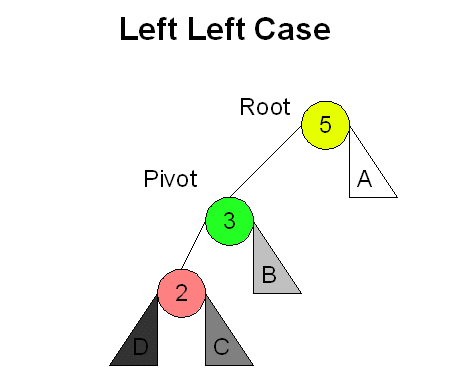
\includegraphics[height=0.8\cardheight]{images/left-left}
}{
  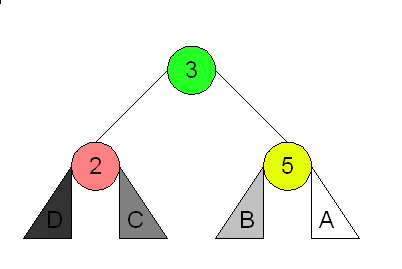
\includegraphics[height=0.8\cardheight]{images/left-left-out}
}

\card{
  What do we do here?\\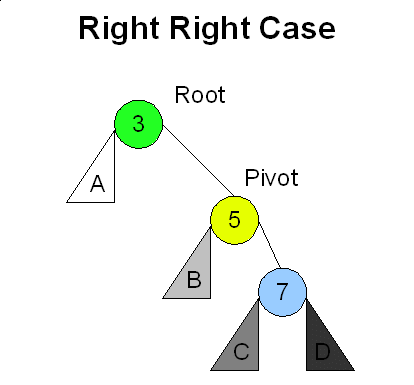
\includegraphics[height=0.8\cardheight]{images/right-right}
}{
  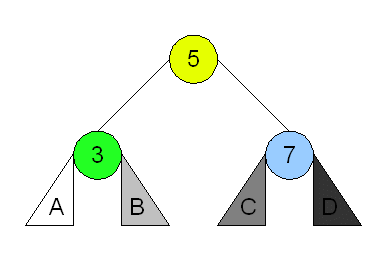
\includegraphics[height=0.8\cardheight]{images/right-right-out}
}

\card{
  What do we do here?\\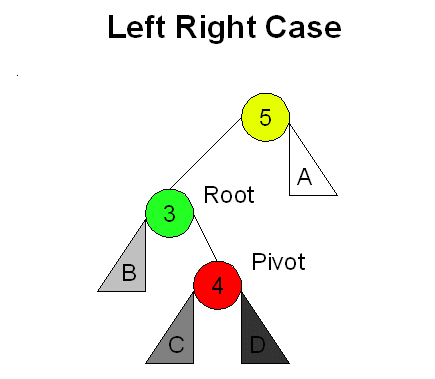
\includegraphics[height=0.8\cardheight]{images/left-right}
}{
  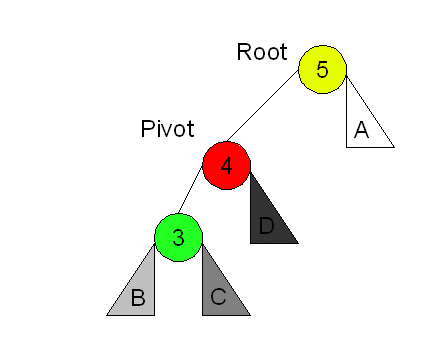
\includegraphics[height=0.8\cardheight]{images/left-right-mid}\\
  Then a left-left!
}

\card{
  What do we do here?\\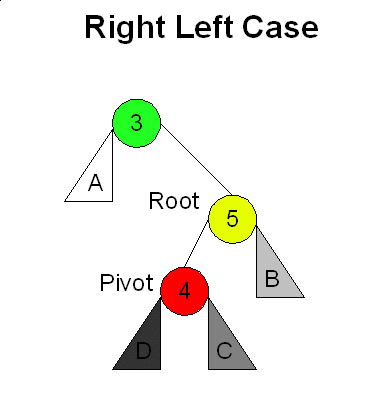
\includegraphics[height=0.8\cardheight]{images/right-left}
}{
  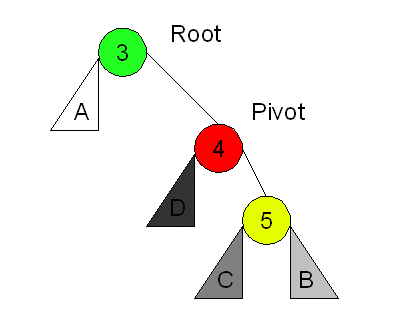
\includegraphics[height=0.8\cardheight]{images/right-left-mid}\\
  Then a right-right!
}

\card{
  What does a Depth First Search use?
}{
  A stack!
}

\card{
  What does a Breadth First Search use?
}{
  A queue!
}

\card{
  What is the running time of Dijkstra's algorithm?
}{
  $O(E + V\log(v))$
}

\card{
  What's the running time of a depth first search when the graph is an adjacency
  matrix?
}{
  $O(V^2)$ since finding neighbours takes $O(V)$ time.
}

\card{
  What's the running time of a depth first search when the graph is an adjacency
  list?
}{
  $O(V + E)$
}

\card{
  How do we insert an element into a heap?
}{
  First, you insert it at the next space in the heap (last element of current
  row, or a new row), then you keep swapping it with its parent if the parent
  is larger than it.
}

\card{
  How do we remove the smallest element from a (min) heap?
}{
  We move the last element from the heap to the first element (we can override
  the first element since we've removed it). Now we `down heap' by swapping
  the moved node with its smallest child until it is smaller than both its
  children or it has no children.
}

\input{semester2-part2.tex}

\end{document}
